

\tikzset{every picture/.style={line width=0.75pt}} %set default line width to 0.75pt        

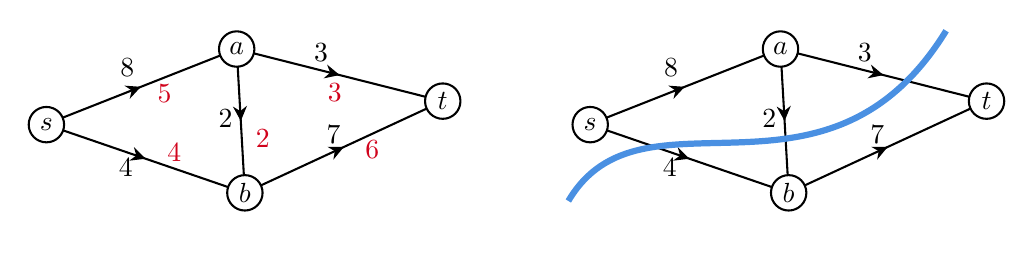
\begin{tikzpicture}[x=0.5pt,y=0.5pt,yscale=-1,xscale=1]
%uncomment if require: \path (0,166); %set diagram left start at 0, and has height of 166

%Straight Lines [id:da3853598268579197] 
\draw    (26.79,81.83) -- (165.31,27.18) ;
\draw [shift={(96.05,54.5)}, rotate = 518.47] [fill={rgb, 255:red, 0; green, 0; blue, 0 }  ][line width=0.08]  [draw opacity=0] (10.72,-5.15) -- (0,0) -- (10.72,5.15) -- (7.12,0) -- cycle    ;
%Straight Lines [id:da14604600957867897] 
\draw    (27.79,81.83) -- (171.22,131.11) ;
\draw [shift={(99.51,106.47)}, rotate = 198.96] [fill={rgb, 255:red, 0; green, 0; blue, 0 }  ][line width=0.08]  [draw opacity=0] (10.72,-5.15) -- (0,0) -- (10.72,5.15) -- (7.12,0) -- cycle    ;
%Straight Lines [id:da8640956582518242] 
\draw    (165.31,27.18) -- (171.22,131.11) ;
\draw [shift={(168.27,79.14)}, rotate = 266.75] [fill={rgb, 255:red, 0; green, 0; blue, 0 }  ][line width=0.08]  [draw opacity=0] (10.72,-5.15) -- (0,0) -- (10.72,5.15) -- (7.12,0) -- cycle    ;
%Straight Lines [id:da285469110869773] 
\draw    (165.31,27.18) -- (314.22,64.84) ;
\draw [shift={(239.76,46.01)}, rotate = 194.2] [fill={rgb, 255:red, 0; green, 0; blue, 0 }  ][line width=0.08]  [draw opacity=0] (10.72,-5.15) -- (0,0) -- (10.72,5.15) -- (7.12,0) -- cycle    ;
%Straight Lines [id:da5085854502811855] 
\draw    (314.22,64.84) -- (171.22,131.11) ;
\draw [shift={(242.72,97.98)}, rotate = 155.13] [fill={rgb, 255:red, 0; green, 0; blue, 0 }  ][line width=0.08]  [draw opacity=0] (10.72,-5.15) -- (0,0) -- (10.72,5.15) -- (7.12,0) -- cycle    ;
%Shape: Ellipse [id:dp651117123053256] 
\draw  [fill={rgb, 255:red, 255; green, 255; blue, 255 }  ,fill opacity=1 ] (15,81.83) .. controls (15,74.77) and (20.73,69.04) .. (27.79,69.04) .. controls (34.86,69.04) and (40.58,74.77) .. (40.58,81.83) .. controls (40.58,88.9) and (34.86,94.62) .. (27.79,94.62) .. controls (20.73,94.62) and (15,88.9) .. (15,81.83) -- cycle ;
%Shape: Ellipse [id:dp7399561756845123] 
\draw  [fill={rgb, 255:red, 255; green, 255; blue, 255 }  ,fill opacity=1 ] (152.52,27.18) .. controls (152.52,20.11) and (158.25,14.39) .. (165.31,14.39) .. controls (172.38,14.39) and (178.1,20.11) .. (178.1,27.18) .. controls (178.1,34.24) and (172.38,39.97) .. (165.31,39.97) .. controls (158.25,39.97) and (152.52,34.24) .. (152.52,27.18) -- cycle ;
%Shape: Ellipse [id:dp8268258265249401] 
\draw  [fill={rgb, 255:red, 255; green, 255; blue, 255 }  ,fill opacity=1 ] (301.43,64.84) .. controls (301.43,57.78) and (307.15,52.05) .. (314.22,52.05) .. controls (321.28,52.05) and (327.01,57.78) .. (327.01,64.84) .. controls (327.01,71.9) and (321.28,77.63) .. (314.22,77.63) .. controls (307.15,77.63) and (301.43,71.9) .. (301.43,64.84) -- cycle ;
%Shape: Ellipse [id:dp5421818862330341] 
\draw  [fill={rgb, 255:red, 255; green, 255; blue, 255 }  ,fill opacity=1 ] (158.43,131.11) .. controls (158.43,124.05) and (164.15,118.32) .. (171.22,118.32) .. controls (178.28,118.32) and (184.01,124.05) .. (184.01,131.11) .. controls (184.01,138.18) and (178.28,143.9) .. (171.22,143.9) .. controls (164.15,143.9) and (158.43,138.18) .. (158.43,131.11) -- cycle ;
%Straight Lines [id:da7732947748811675] 
\draw    (419.79,81.83) -- (558.31,27.18) ;
\draw [shift={(489.05,54.5)}, rotate = 518.47] [fill={rgb, 255:red, 0; green, 0; blue, 0 }  ][line width=0.08]  [draw opacity=0] (10.72,-5.15) -- (0,0) -- (10.72,5.15) -- (7.12,0) -- cycle    ;
%Straight Lines [id:da1657956393922747] 
\draw    (420.79,81.83) -- (564.22,131.11) ;
\draw [shift={(492.51,106.47)}, rotate = 198.96] [fill={rgb, 255:red, 0; green, 0; blue, 0 }  ][line width=0.08]  [draw opacity=0] (10.72,-5.15) -- (0,0) -- (10.72,5.15) -- (7.12,0) -- cycle    ;
%Straight Lines [id:da624664652241142] 
\draw    (558.31,27.18) -- (564.22,131.11) ;
\draw [shift={(561.27,79.14)}, rotate = 266.75] [fill={rgb, 255:red, 0; green, 0; blue, 0 }  ][line width=0.08]  [draw opacity=0] (10.72,-5.15) -- (0,0) -- (10.72,5.15) -- (7.12,0) -- cycle    ;
%Straight Lines [id:da16414400972514853] 
\draw    (558.31,27.18) -- (707.22,64.84) ;
\draw [shift={(632.76,46.01)}, rotate = 194.2] [fill={rgb, 255:red, 0; green, 0; blue, 0 }  ][line width=0.08]  [draw opacity=0] (10.72,-5.15) -- (0,0) -- (10.72,5.15) -- (7.12,0) -- cycle    ;
%Straight Lines [id:da25842435999681035] 
\draw    (707.22,64.84) -- (564.22,131.11) ;
\draw [shift={(635.72,97.98)}, rotate = 155.13] [fill={rgb, 255:red, 0; green, 0; blue, 0 }  ][line width=0.08]  [draw opacity=0] (10.72,-5.15) -- (0,0) -- (10.72,5.15) -- (7.12,0) -- cycle    ;
%Shape: Ellipse [id:dp4665458374254806] 
\draw  [fill={rgb, 255:red, 255; green, 255; blue, 255 }  ,fill opacity=1 ] (408,81.83) .. controls (408,74.77) and (413.73,69.04) .. (420.79,69.04) .. controls (427.86,69.04) and (433.58,74.77) .. (433.58,81.83) .. controls (433.58,88.9) and (427.86,94.62) .. (420.79,94.62) .. controls (413.73,94.62) and (408,88.9) .. (408,81.83) -- cycle ;
%Shape: Ellipse [id:dp05678239039201238] 
\draw  [fill={rgb, 255:red, 255; green, 255; blue, 255 }  ,fill opacity=1 ] (545.52,27.18) .. controls (545.52,20.11) and (551.25,14.39) .. (558.31,14.39) .. controls (565.38,14.39) and (571.1,20.11) .. (571.1,27.18) .. controls (571.1,34.24) and (565.38,39.97) .. (558.31,39.97) .. controls (551.25,39.97) and (545.52,34.24) .. (545.52,27.18) -- cycle ;
%Shape: Ellipse [id:dp6844281882371538] 
\draw  [fill={rgb, 255:red, 255; green, 255; blue, 255 }  ,fill opacity=1 ] (694.43,64.84) .. controls (694.43,57.78) and (700.15,52.05) .. (707.22,52.05) .. controls (714.28,52.05) and (720.01,57.78) .. (720.01,64.84) .. controls (720.01,71.9) and (714.28,77.63) .. (707.22,77.63) .. controls (700.15,77.63) and (694.43,71.9) .. (694.43,64.84) -- cycle ;
%Shape: Ellipse [id:dp4715996456353091] 
\draw  [fill={rgb, 255:red, 255; green, 255; blue, 255 }  ,fill opacity=1 ] (551.43,131.11) .. controls (551.43,124.05) and (557.15,118.32) .. (564.22,118.32) .. controls (571.28,118.32) and (577.01,124.05) .. (577.01,131.11) .. controls (577.01,138.18) and (571.28,143.9) .. (564.22,143.9) .. controls (557.15,143.9) and (551.43,138.18) .. (551.43,131.11) -- cycle ;
%Curve Lines [id:da9207367536031942] 
\draw [color={rgb, 255:red, 74; green, 144; blue, 226 }  ,draw opacity=1 ][line width=2.25]    (405,137) .. controls (458,47) and (591,155) .. (678,14) ;

% Text Node
\draw (27.79,81.83) node   [align=left] {$\displaystyle s$};
% Text Node
\draw (165.31,27.18) node   [align=left] {$\displaystyle a$};
% Text Node
\draw (314.22,64.84) node   [align=left] {$\displaystyle t$};
% Text Node
\draw (171.22,131.11) node   [align=left] {$\displaystyle b$};
% Text Node
\draw (229,50) node [anchor=north west][inner sep=0.75pt]   [align=left] {$\displaystyle \textcolor[rgb]{0.82,0.01,0.11}{3}$};
% Text Node
\draw (79,32) node [anchor=north west][inner sep=0.75pt]   [align=left] {$\displaystyle 8$};
% Text Node
\draw (228,80) node [anchor=north west][inner sep=0.75pt]   [align=left] {$\displaystyle 7$};
% Text Node
\draw (150,69) node [anchor=north west][inner sep=0.75pt]   [align=left] {$\displaystyle 2$};
% Text Node
\draw (256,91) node [anchor=north west][inner sep=0.75pt]   [align=left] {$\displaystyle \textcolor[rgb]{0.82,0.01,0.11}{6}$};
% Text Node
\draw (177,83) node [anchor=north west][inner sep=0.75pt]   [align=left] {$\displaystyle \textcolor[rgb]{0.82,0.01,0.11}{2}$};
% Text Node
\draw (219,21) node [anchor=north west][inner sep=0.75pt]   [align=left] {$\displaystyle 3$};
% Text Node
\draw (106,51) node [anchor=north west][inner sep=0.75pt]   [align=left] {$\displaystyle \textcolor[rgb]{0.82,0.01,0.11}{5}$};
% Text Node
\draw (78,104) node [anchor=north west][inner sep=0.75pt]   [align=left] {$\displaystyle 4$};
% Text Node
\draw (113,93) node [anchor=north west][inner sep=0.75pt]   [align=left] {$\displaystyle \textcolor[rgb]{0.82,0.01,0.11}{4}$};
% Text Node
\draw (420.79,81.83) node   [align=left] {$\displaystyle s$};
% Text Node
\draw (558.31,27.18) node   [align=left] {$\displaystyle a$};
% Text Node
\draw (707.22,64.84) node   [align=left] {$\displaystyle t$};
% Text Node
\draw (564.22,131.11) node   [align=left] {$\displaystyle b$};
% Text Node
\draw (472,32) node [anchor=north west][inner sep=0.75pt]   [align=left] {$\displaystyle 8$};
% Text Node
\draw (621,80) node [anchor=north west][inner sep=0.75pt]   [align=left] {$\displaystyle 7$};
% Text Node
\draw (543,69) node [anchor=north west][inner sep=0.75pt]   [align=left] {$\displaystyle 2$};
% Text Node
\draw (612,21) node [anchor=north west][inner sep=0.75pt]   [align=left] {$\displaystyle 3$};
% Text Node
\draw (471,104) node [anchor=north west][inner sep=0.75pt]   [align=left] {$\displaystyle 4$};


\end{tikzpicture}

